\documentclass[a4wide]{report}

\usepackage{amsmath}
\usepackage[a4paper, total={7in, 10.2in}]{geometry}
\usepackage{graphicx}
\usepackage[portuguese]{babel}
\usepackage[utf8]{inputenc}


\begin{document}

\noindent
{\bf Rafael V. Cacilhas  - Relatório 10 (\today)}

\vspace{0.5cm}

\section*{Exercício 1}

\subsection*{a) }
Na Figura \ref{1a} foi feito uma sequência de 100 número aleatórios. Em seguida, em outro software, foi feito uma sequência de 50 números aleatorios; note que os primeiros 50 números são idênticos, o que mostra que o gerador de número aleatórios sempre gera os mesmos números caso não seja iniciado com uma $\textit{seed}$ específica. Por fim, o estado do gerador foi salvo e carregado em um terceiro programa, que gerou mais 50 números aleatórios. Note que eles coincidem com os últimos 50 números da sequência direta, o que evidencia que é possivel salvar e começar o gerador do ponto desejado.

\begin{figure}[!htb]
\centering
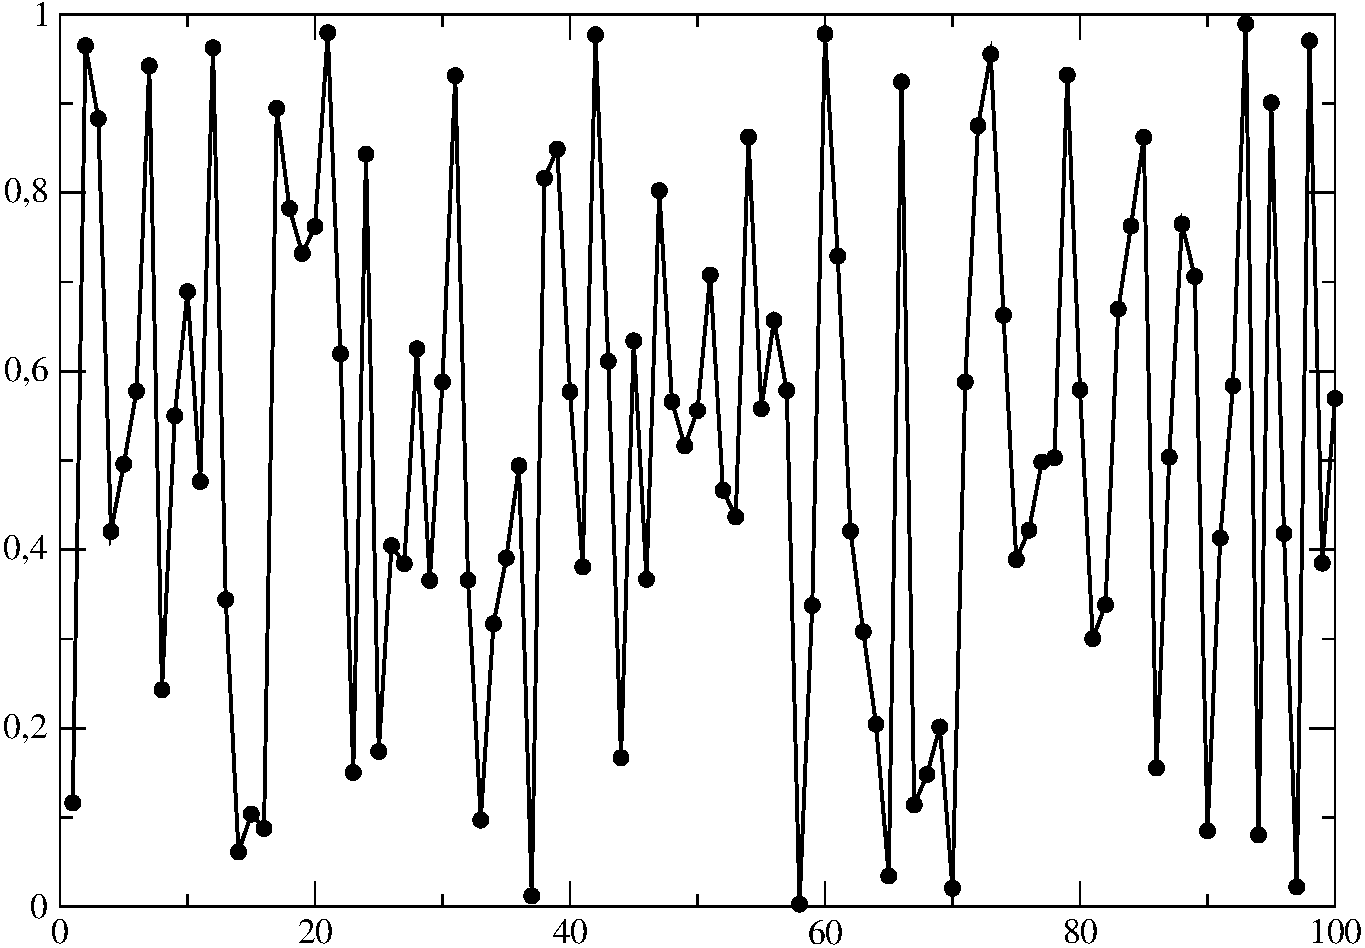
\includegraphics[width=0.32\textwidth]{sequencia_direta.pdf}
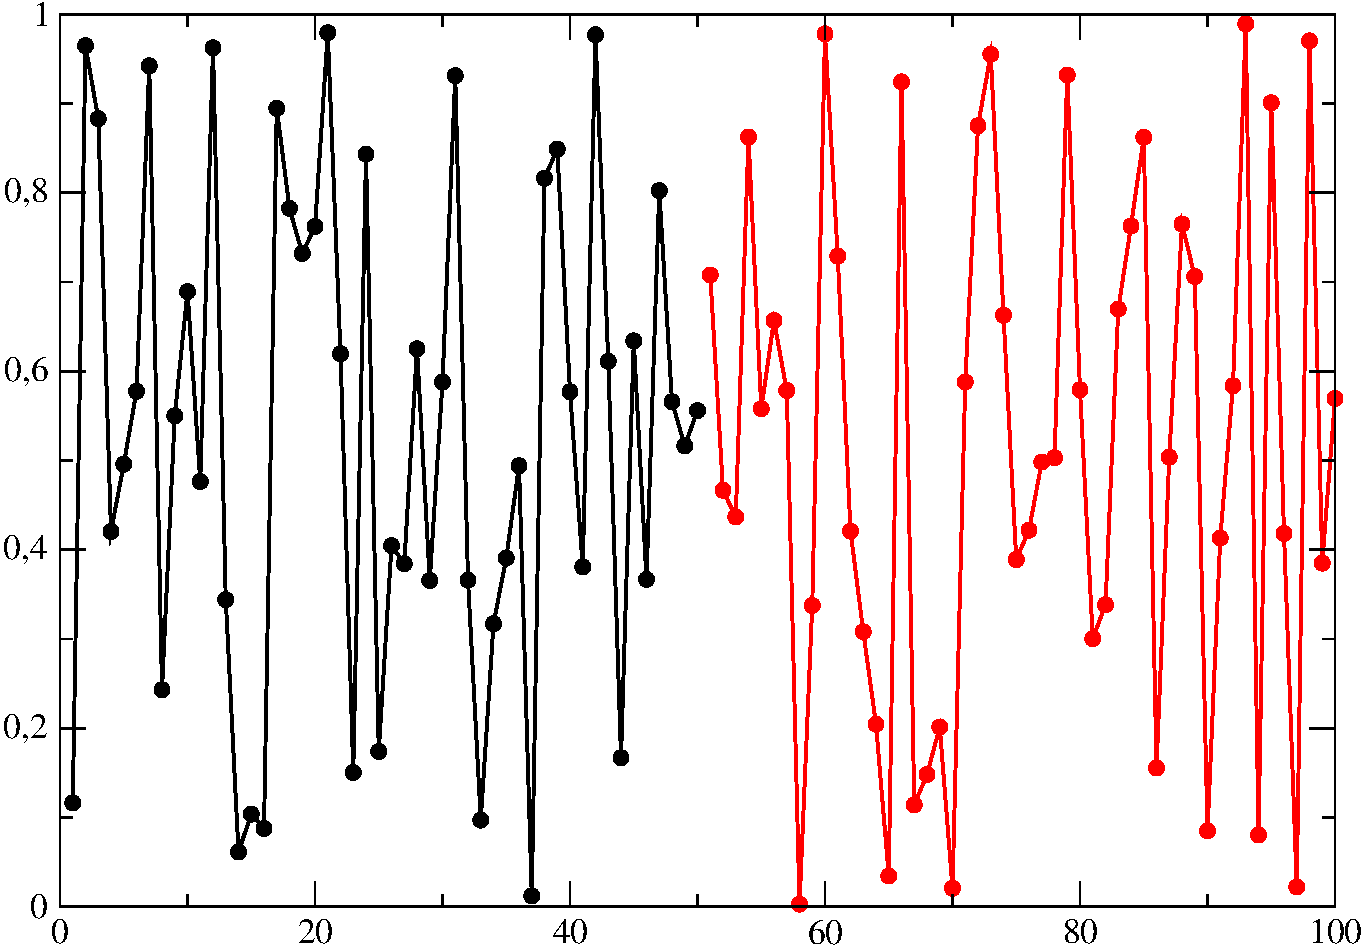
\includegraphics[width=0.32\textwidth]{sequencia_meio2.pdf}
\caption{Sequência de 100 números aleatórios gerados initerruptamente (esquerda) e sequência de 50 números seguidos de outros 50 números (direita).}
\label{1a}
\end{figure}




\subsection*{b) }

Na Figura \ref{1b} é possível ver os histogramas para $N =10^3$,$N =10^4$, e $N =10^6$, respectivamente. Note como os números aleatórios gerados seguem uma distribuição constante no intervalo [0,1]. O fato da distribuição não ser perfeitamente constante é devido a quantidade de números gerados não ser infinita, visto que a distribuição passa a ser cada vez mais constante com o aumento de números gerados. 


\begin{figure}[!htb]
\centering
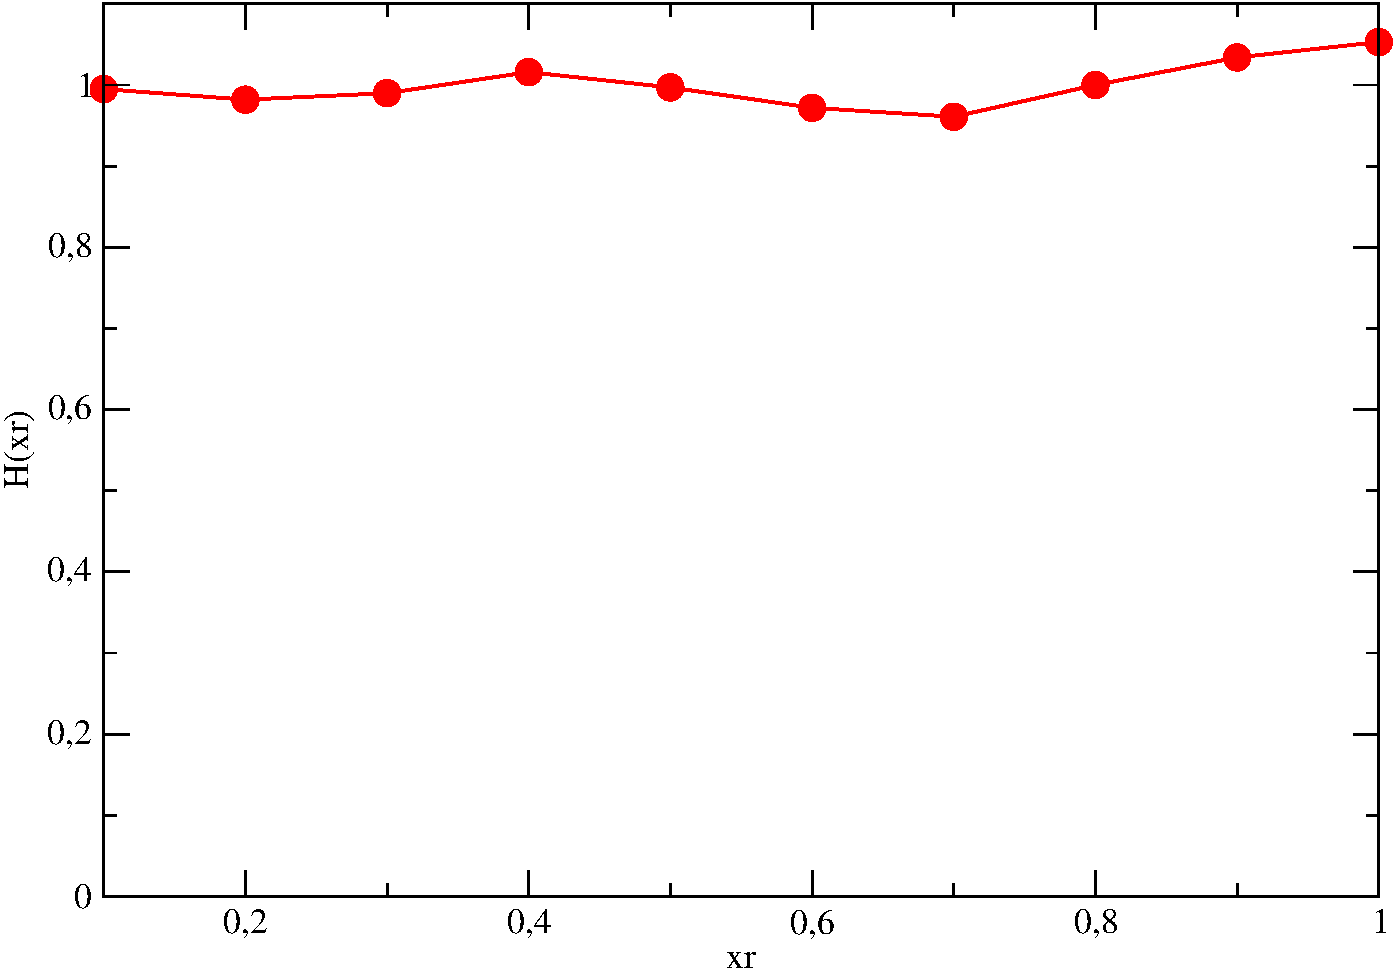
\includegraphics[width=0.32\textwidth]{103.pdf}
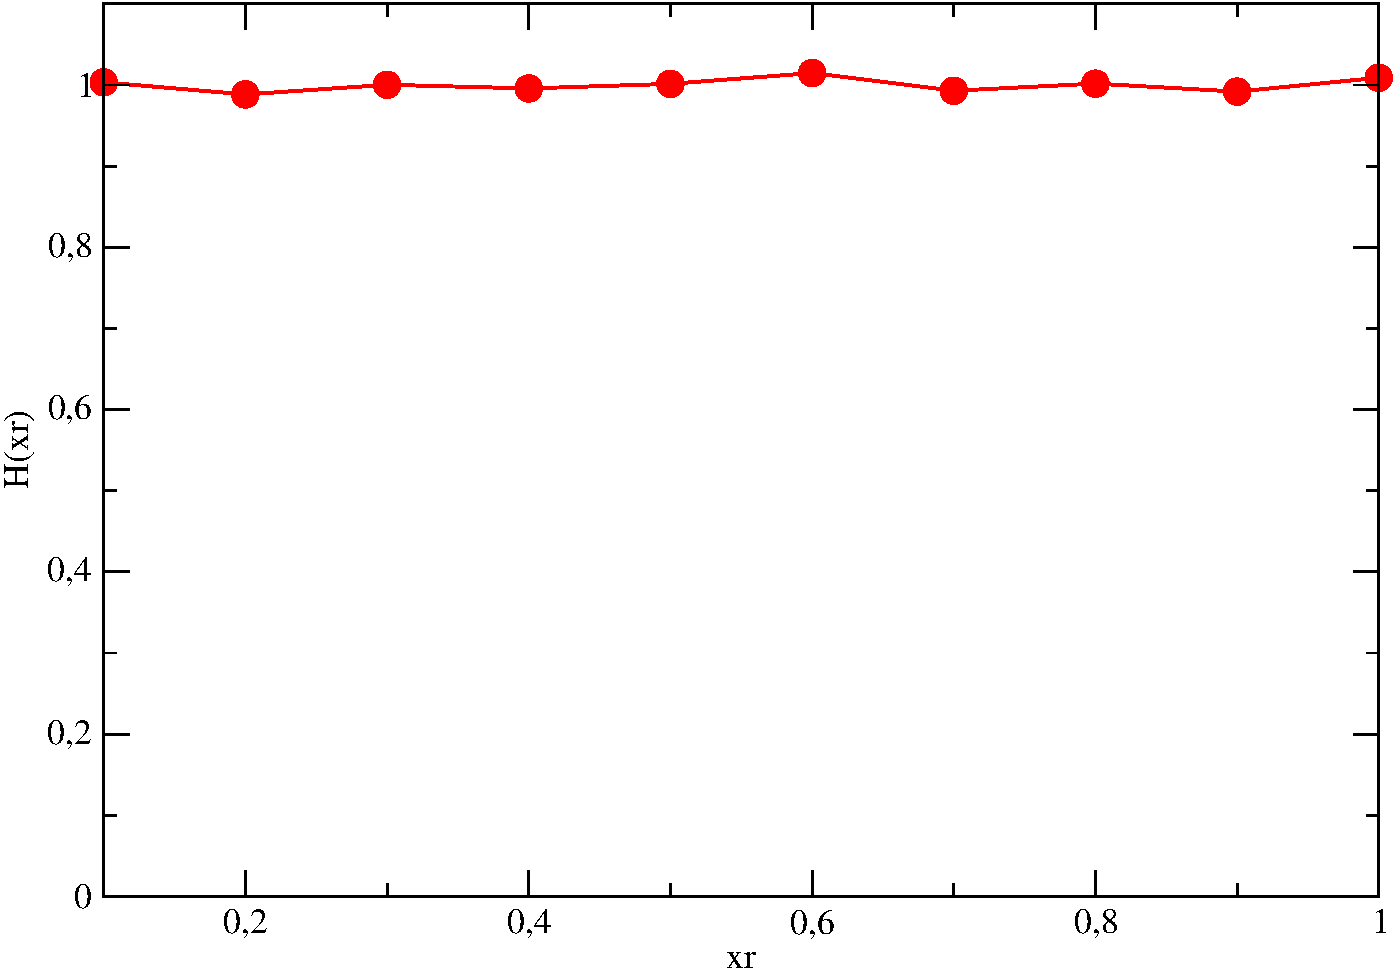
\includegraphics[width=0.32\textwidth]{104.pdf}
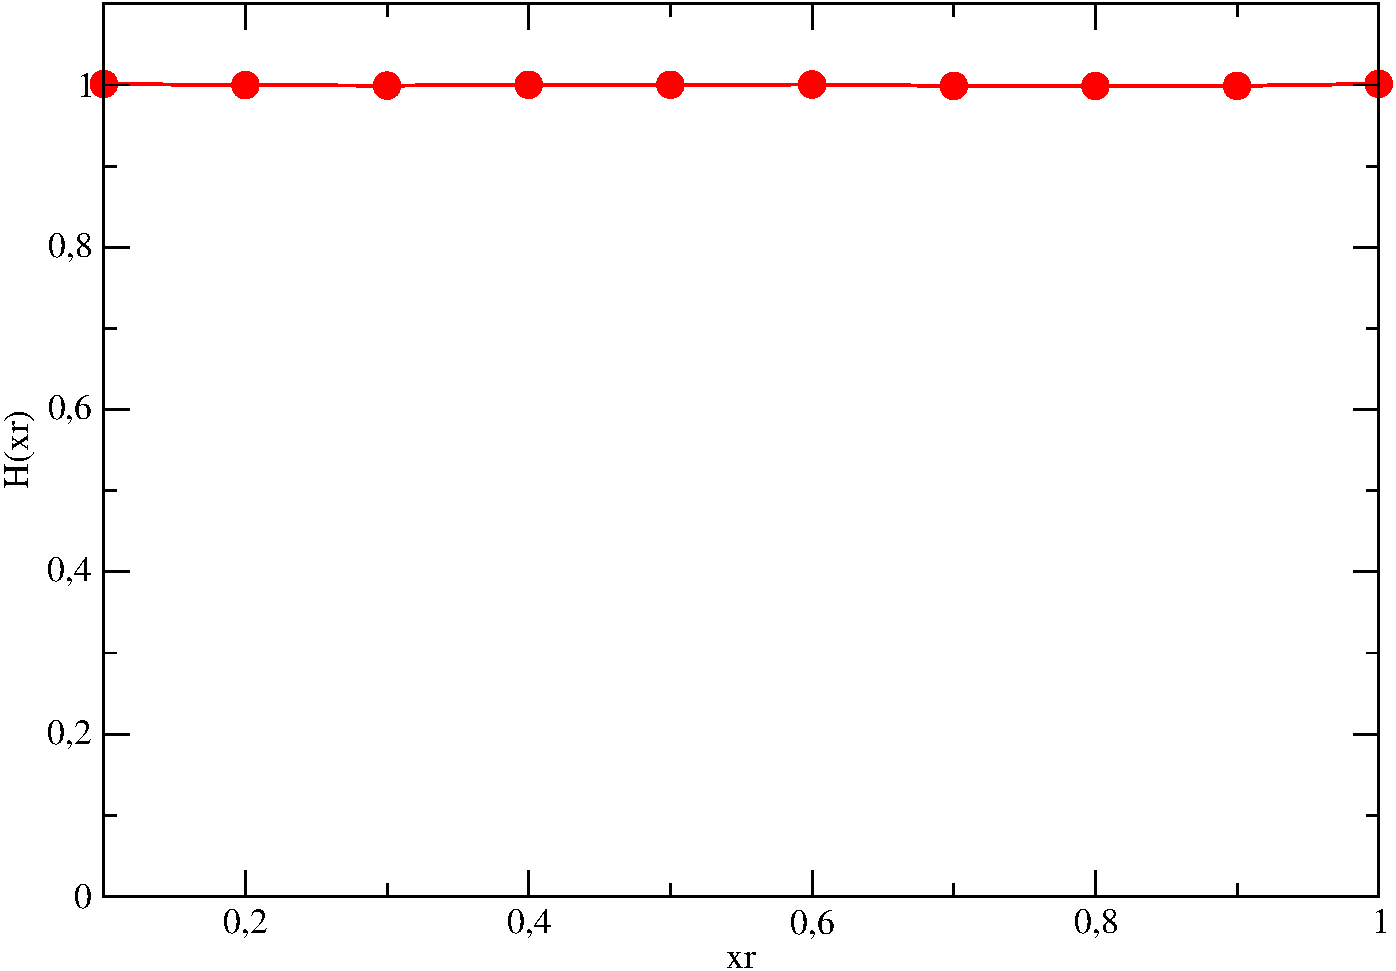
\includegraphics[width=0.32\textwidth]{106.pdf}
\caption{Histograma dos números aleatórios gerados para $N =10^3$ (esquerda),$N =10^4$ (meio) e $N =10^6$ (direita).}
\label{1b}
\end{figure}

\subsection*{c) }

Na Figura \ref{1c} temos a auto-correlação C(i) para i entre 0 e 30. Note que C(i) possui valores menores do que 1, o que evidencia que os números aleatórios são completamente descorrelacionados. Ainda na Figura \ref{1c} temos o tempo de auto-correlação integrado $2\tau_{int}$.

\begin{figure}[!htb]
\centering
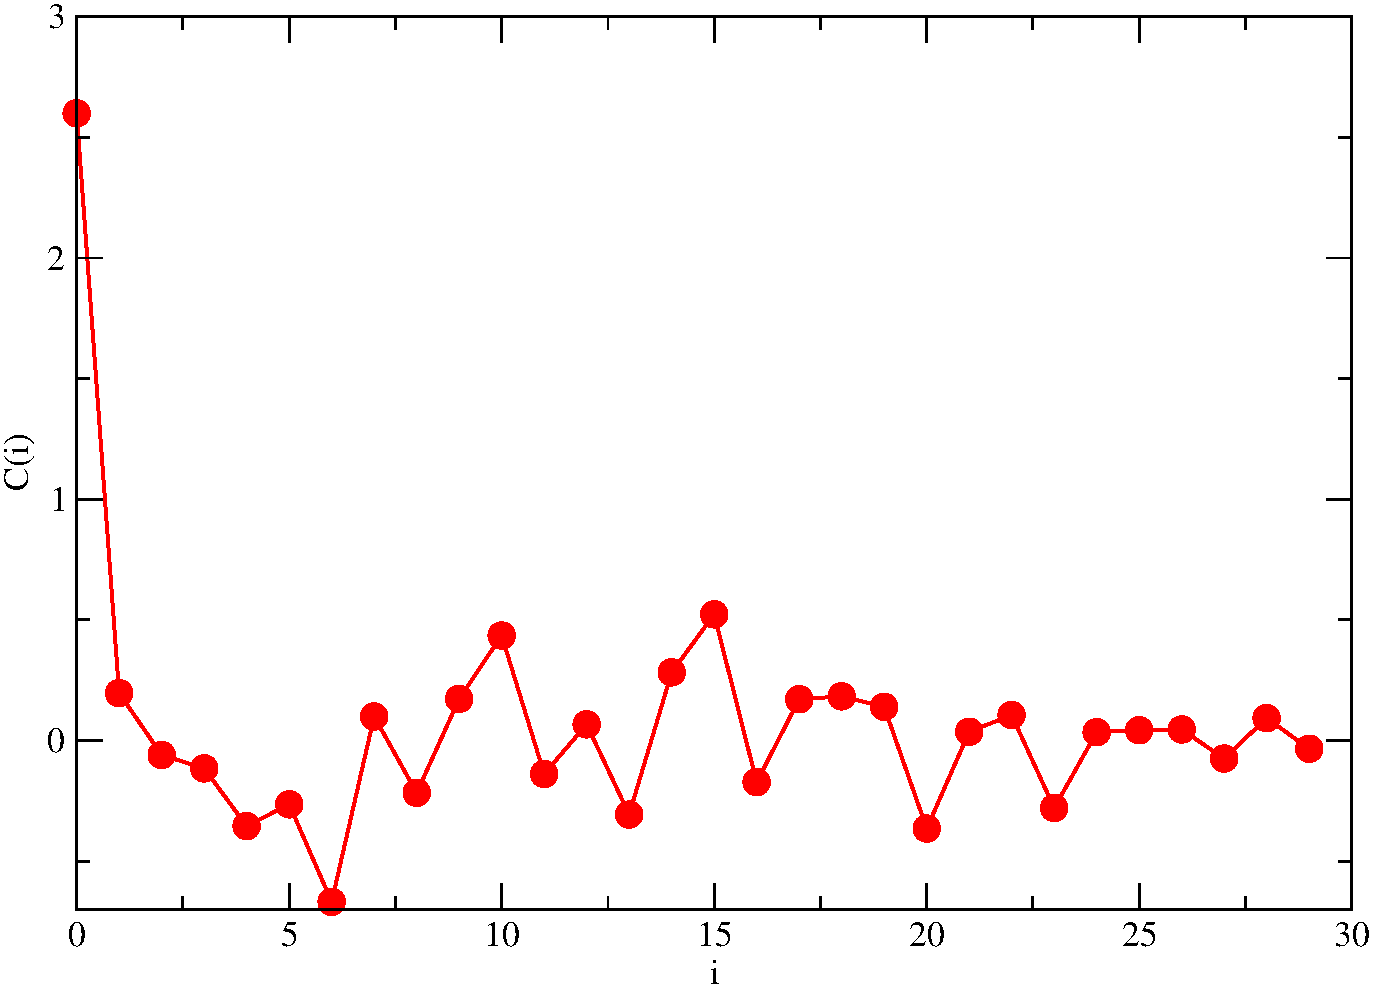
\includegraphics[width=0.32\textwidth]{Ci.pdf}
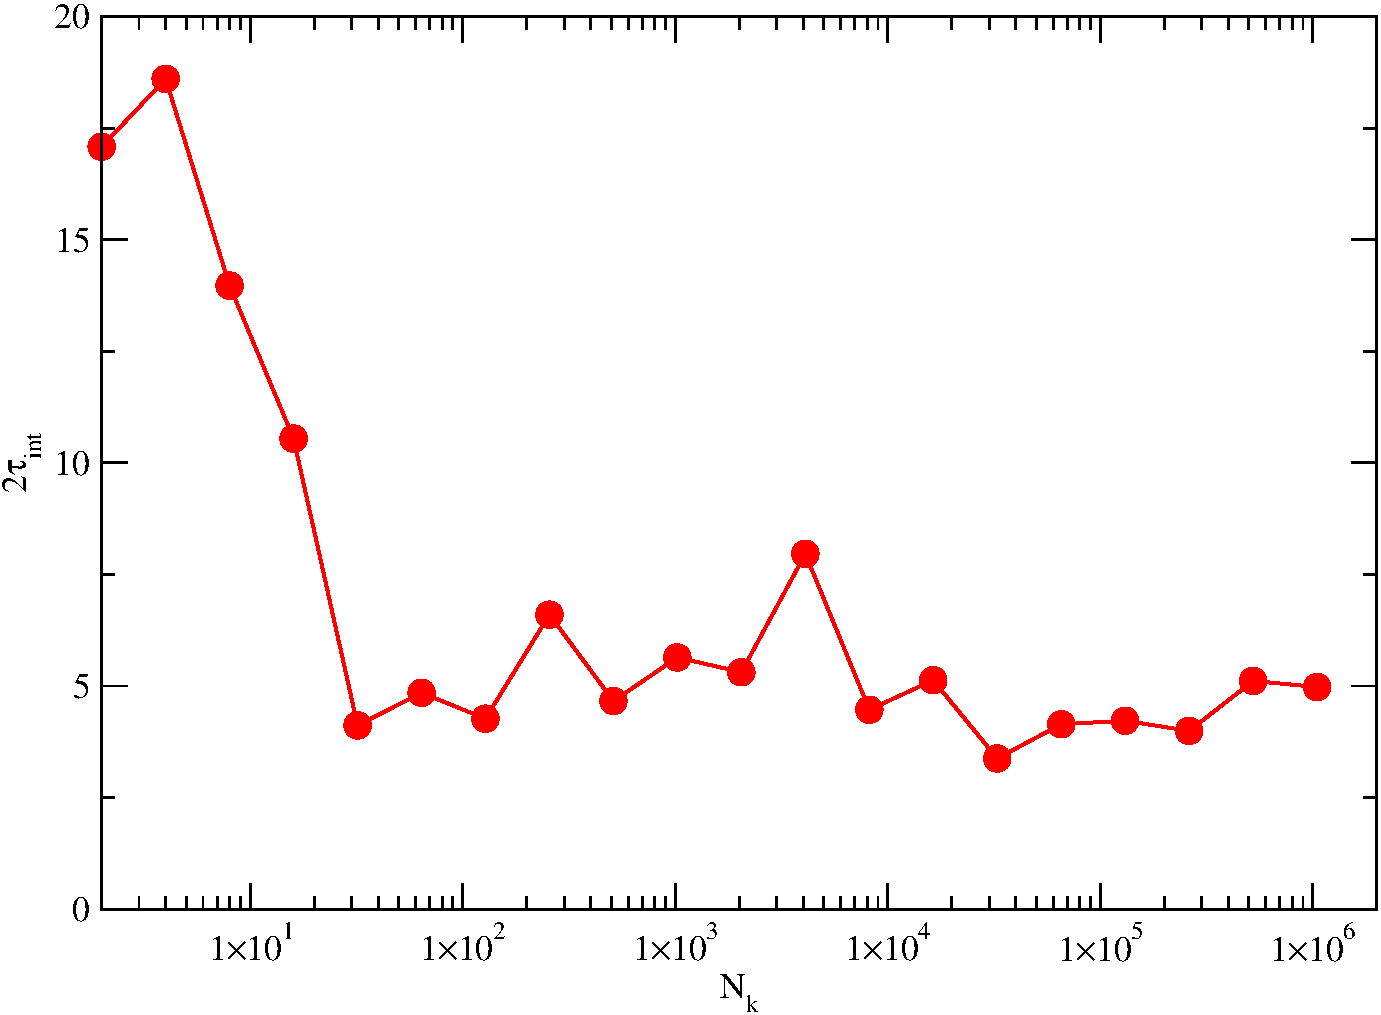
\includegraphics[width=0.32\textwidth]{tau.pdf}
\caption{Auto-correlação C(i) (esquerda) e tempo de auto-correlação integrado $2\tau$ (direita).}
\label{1c}
\end{figure}


\section*{Exercício 2}

\subsection*{a)}
A média $\bar{x}$ e o desvio padrão $\sigma^2$ calculados são $4.19 \pm 5.04$, respectivamente. Se observarmos a Figura \ref{2a} podemos ver que os números de fato parecem estar distribuidos com média perto de 4 e que a maioria dos números se encontra no intervalo [0,8], o que evidencia que a média e desvio padrão calculados estão condizentes.

\begin{figure}[!htb]
\centering
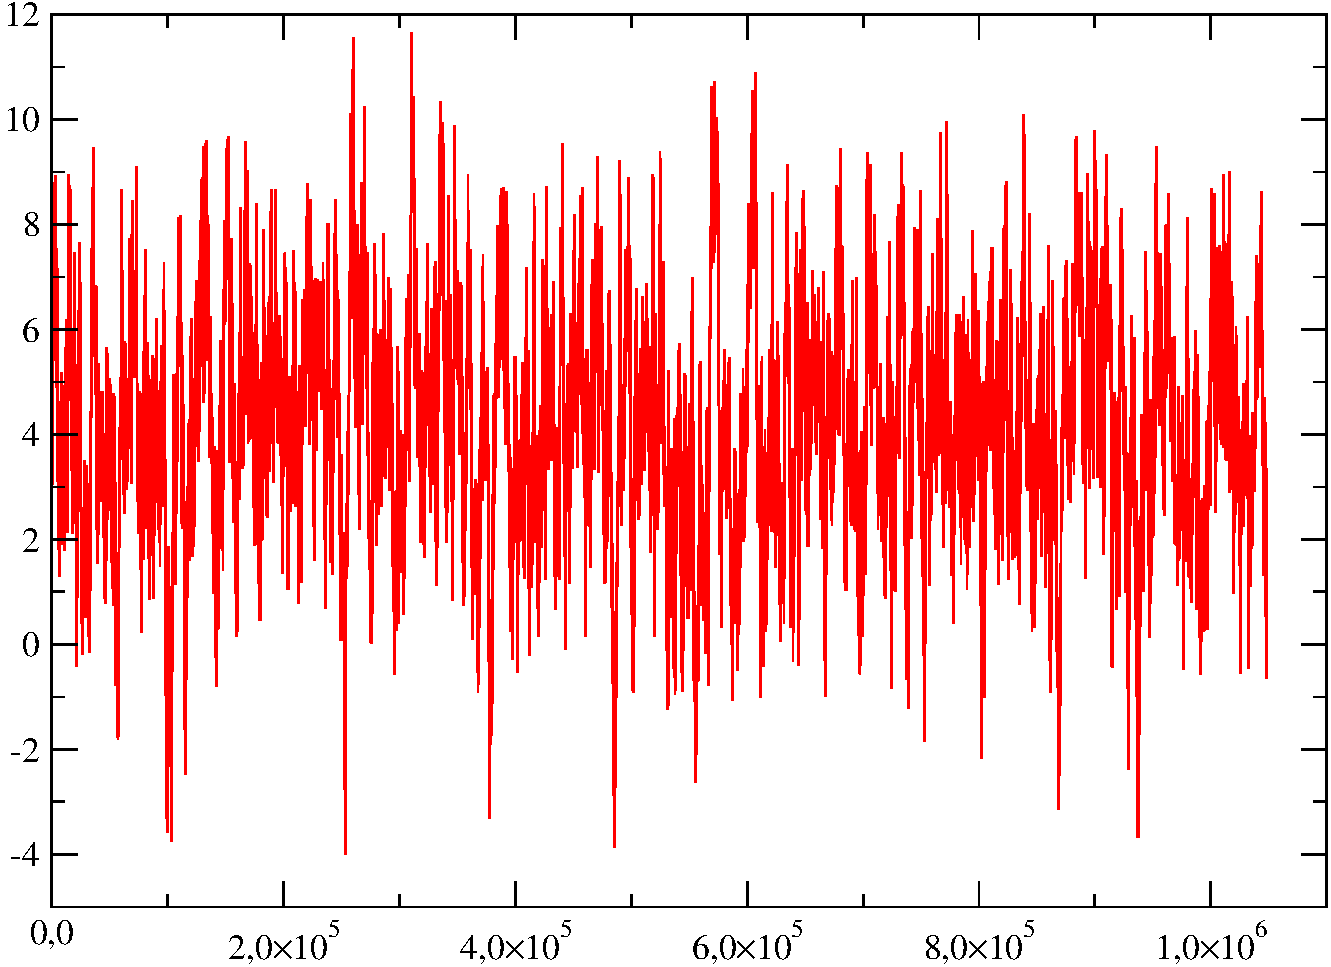
\includegraphics[width=0.32\textwidth]{saida.pdf}
\caption{Sequência de número aleatórios lidos.}
\label{2a}
\end{figure}


\section*{Exercício 3}
\subsection*{a)}
A subrotina está no programa \textit{gas.f90}. As condições iniciais geradas podem ser vistas na Figura \ref{3a}, onde pode ser visto uma distribuição contínua na posição e uma gaussiana para a componente x da velocidade. A componente y da velocidade foi otimitida pois não há motivos para ser diferente da componente x. Como discutido no exercício 1 o fato das distribuições não serem perfeitamente constante e gaussiana é devido ao fato de que o número de partículas não é infinito.
\begin{figure}[!htb]
\centering
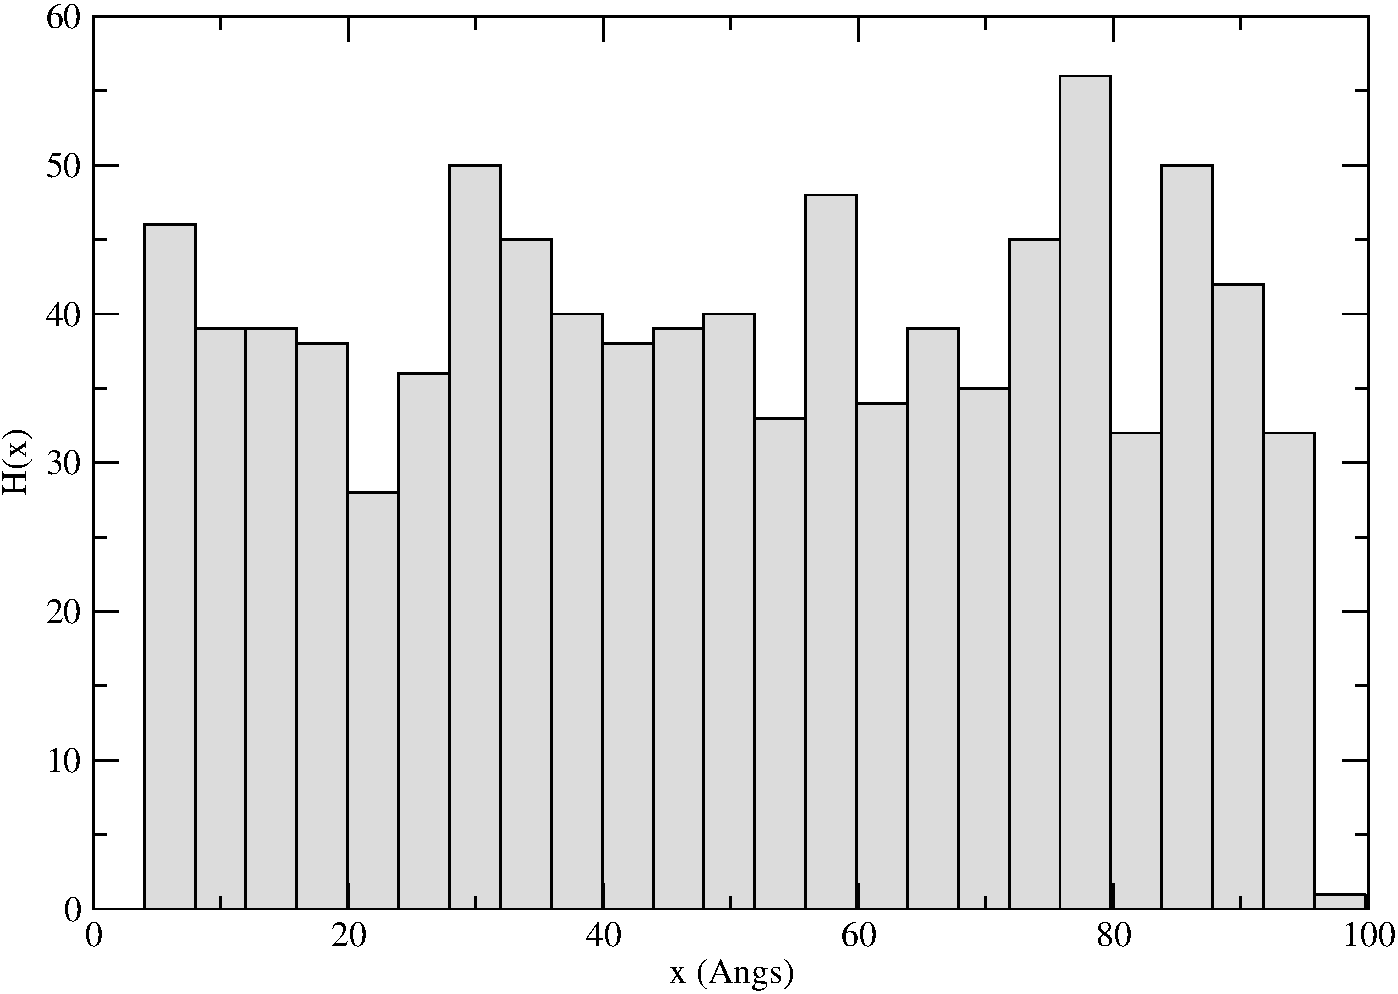
\includegraphics[width=0.32\textwidth]{histogramax.pdf}
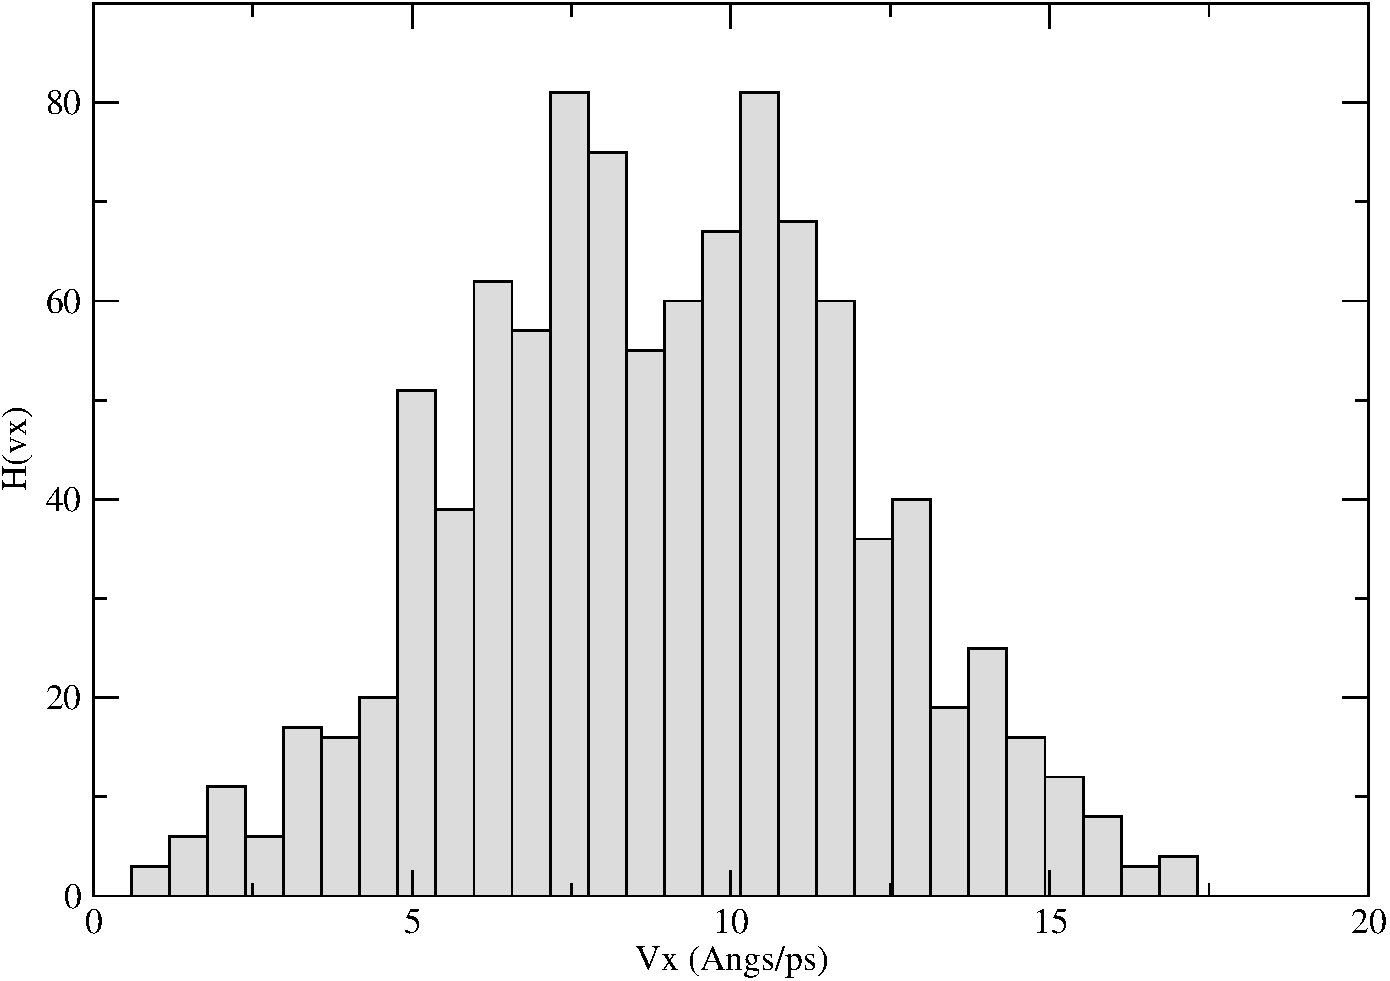
\includegraphics[width=0.32\textwidth]{histogramavx.pdf}
\caption{Condições iniciais geradas.}
\label{3a}
\end{figure}

\subsection*{b)}
A energia cinética total do sistema pode ser vista na Figura \ref{3b}. Há uma queda na energia cinética total para tempos curtos, mas a energia cinética inicial é gradativamente recuperada em tempos longos.

\begin{figure}[!htb]
\centering
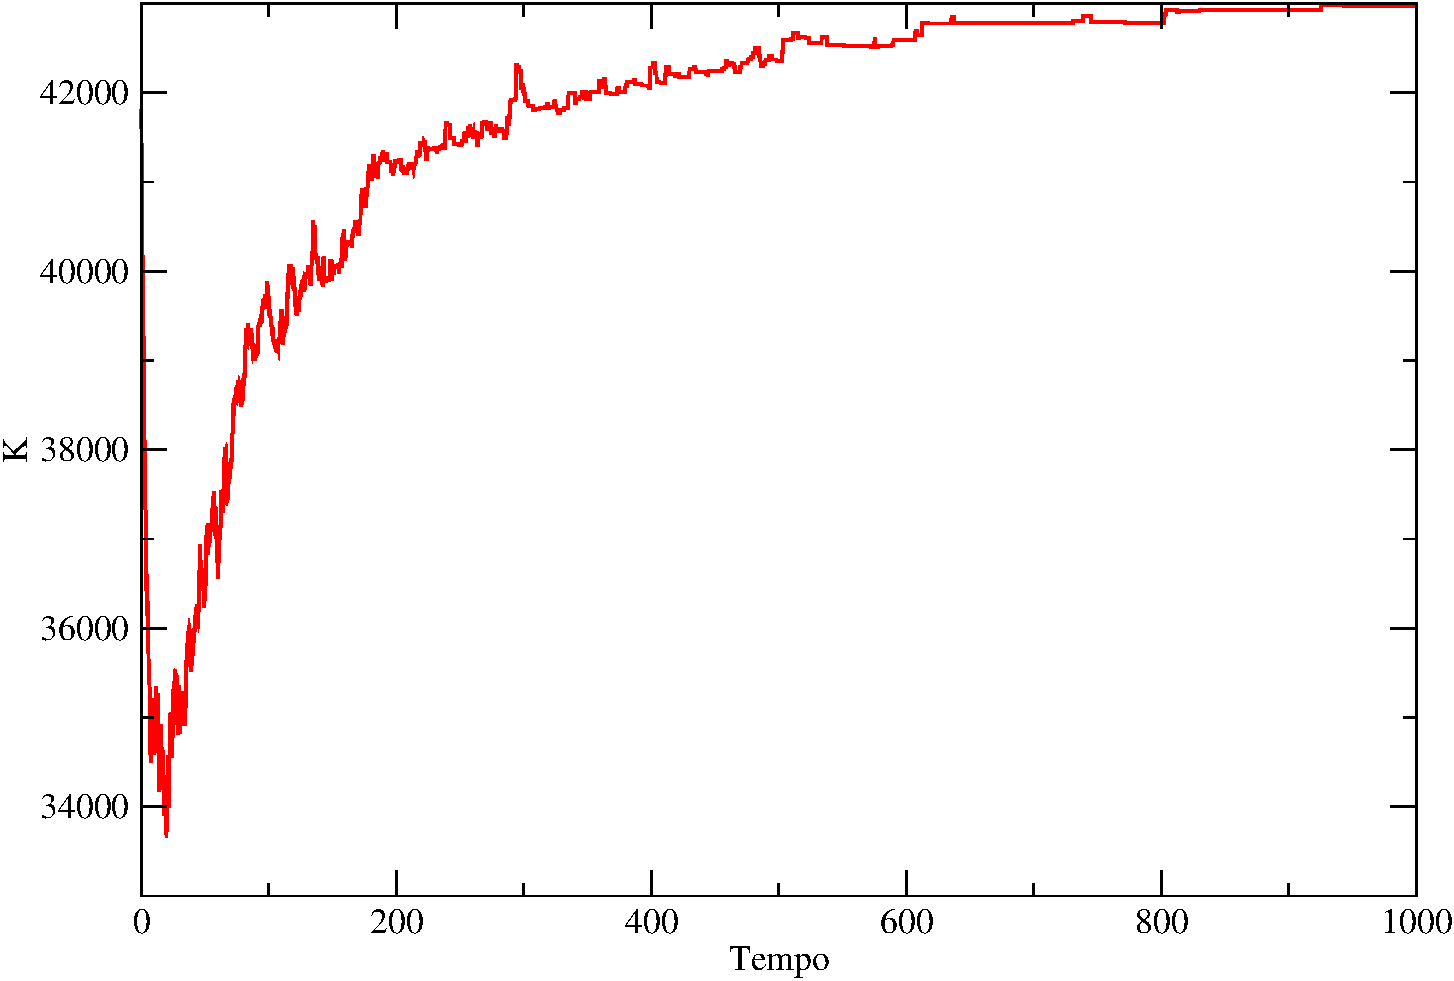
\includegraphics[width=0.32\textwidth]{k.pdf}
\caption{Energia cinética total em função do tempo.}
\label{3b}
\end{figure}

\subsection*{c)}
A teoria cinética dos gases prevê que a a razão entre a média da velocidade e a média quadrática é:
\begin{equation}
\frac{\bar{v}_{rms}}{\bar{|v|}} = \sqrt{\frac{\pi}{2}}
\end{equation}

Na Figura \ref{3c} podemos ver que a razão entre as duas médias é constante.

\begin{figure}[!htb]
\centering
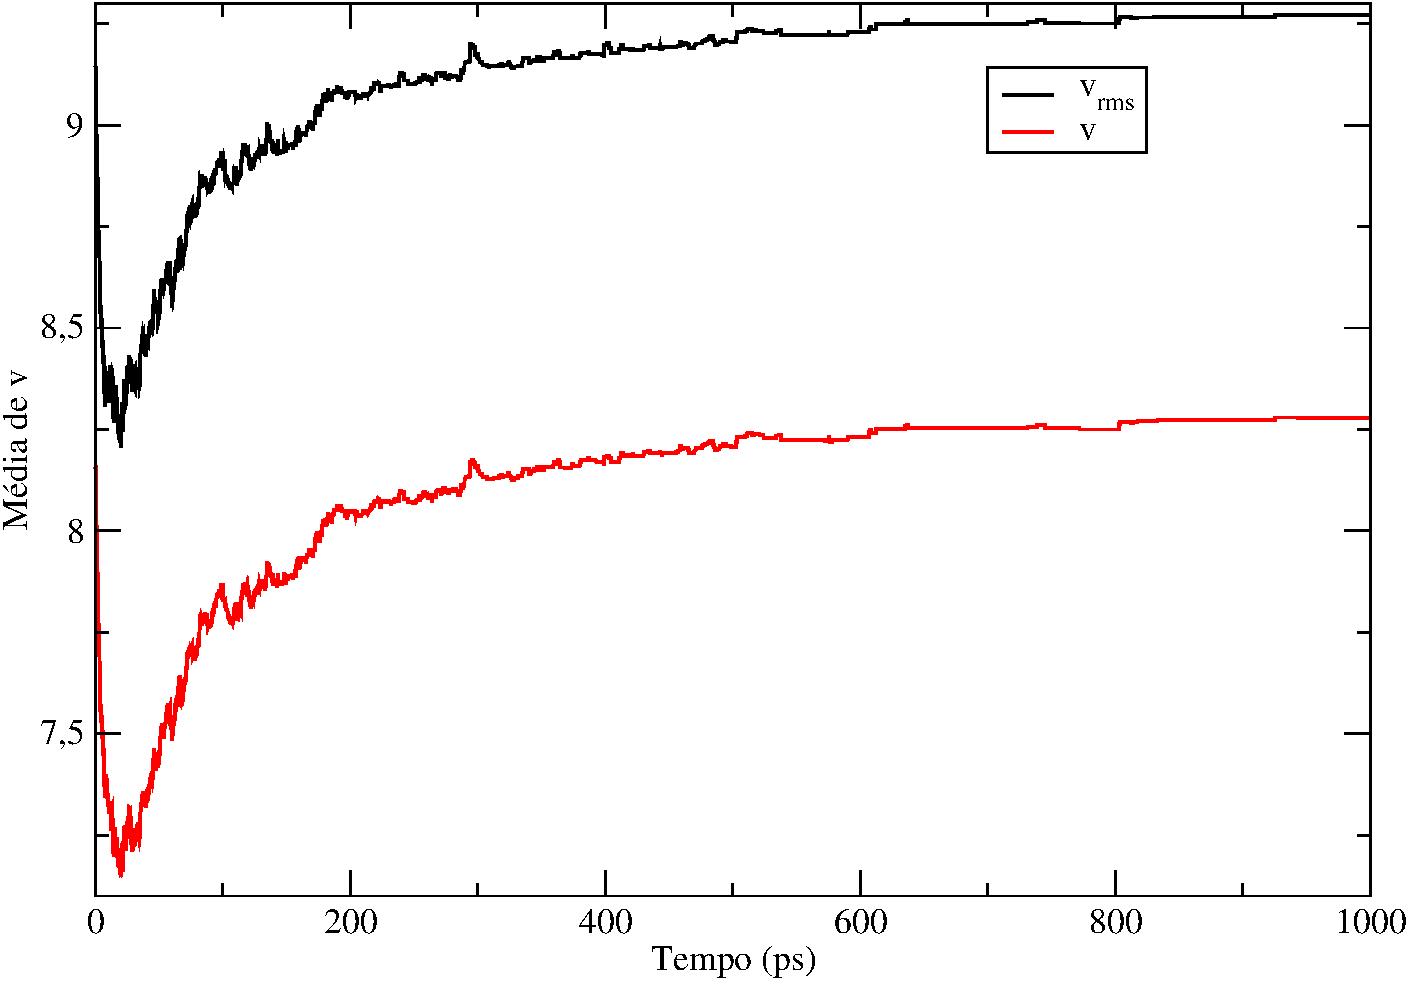
\includegraphics[width=0.32\textwidth]{medias.pdf}
\caption{Condições iniciais geradas.}
\label{3c}
\end{figure}

\section*{Exercício 4}

O programa começou a ser feito e pode ser conferido em sua respectiva pasta. Infelizmente não houve tempo para finalizar e gerar os dados pedidos.






\end{document}